In questa sezione verranno elencati ed analizzati tutti i casi d'uso$^*$ individuati dal gruppo. Ogni caso d'uso verrà identificato da un codice univoco secondo le regole descritte nel documento \textit{Norme di progetto} e riportate di seguito. 
\subsection{Denominazione dei casi d'uso}
Ad ogni caso d'uso saranno associate le seguenti informazioni:
\begin{itemize}
\item il codice del requisito che lo interessa UC-[Codice];
\item un nome (univoco);
\item le pre-condizioni e le post-condizioni relative allo specifico caso d'uso;
\item gli attori coinvolti, sia primari che secondari;
\item lo scenario principale che il caso d'uso vorrebbe modellare;
\item le eventuali estensioni dello scenario principale.
\end{itemize}

\subsubsection{Gerarchie dei casi d'uso} 

Gli identificatori numerici assegnati a casi d'uso saranno organizzati gerarchicamente. Posto UC-X codice di un caso d'uso, allora UC-X.Y è figlio di UC-X ed esiste fra i due una relazione tra quelle elencate:
\begin{itemize}
\item UC-X.Y descrive nel dettaglio una delle funzionalita di UC-X;
\item UC-X.Y descrive una estensione (o scenario alternativo) dello scenario descritto in UC-X; 
\item UC-X.Y descrive una estensione dello scenario principale di due o più figli di UC-X.
\end{itemize}

\subsection{Elenco dei casi d'uso}
\subsubsection{UC-1 Registrazione}
\begin{figure}[h]
	\centering
	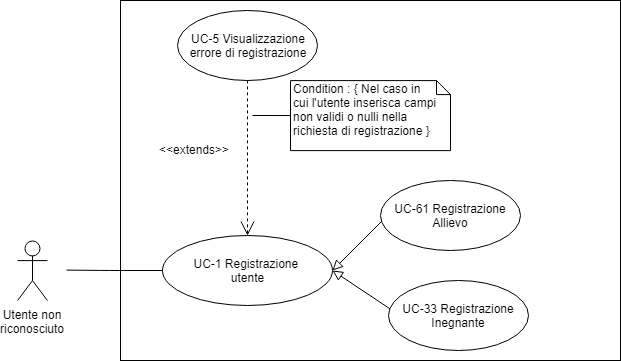
\includegraphics[scale=0.7]{images/UC-1.png}
	\caption{UC-1 Registrazione}
\end{figure}	

\begin{itemize}
		\item \textbf{Attori: }Utente non registrato.
		\item \textbf{Precondizione: }L'utente si trova nella vista di registrazione dell'applicazione.
		\item \textbf{Postcondizione: }L'utente è registrato o come allievo o come insegnante.
		\item \textbf{Scenario principale: }
		\begin{enumerate}
		\item L'utente ha scelto di registrarsi al sistema, quindi di creare un nuovo profilo. 
		\item L'utente dovrà scegliere la tipologia di utente, insegnante/allievo. 
		\item L'utente inserirà nome, cognome, username, email e password.
		\item L'utente fornirà il nome della scuola a cui appartiene e la città.
		\item L'utente conferma la registrazione.
		\end{enumerate}
		\item \textbf{Estensioni: }
		\begin{itemize}
			\item 5.a Nel caso in cui l'utente tenti l'inserimento di campi non validi vedrà comparire dei messaggi d'errore (UC-5).
			\item 5.b Un utente che si è registrato come insegnante deve attendere la conferma dela registrazione del moderatore (UC-4).
			\item 5.c Un utente che invia la domanda di registrazione deve confermare o annullare l'operazione (UC-32).
		\end{itemize}
	\end{itemize}
\subsubsection{UC-2 Autenticazione}
		\begin{itemize}
			\item \textbf{Attori:} Utente non autenticato.
			\item \textbf{Precondizione:} L'utente si trova nella vista di autenticazione dell'applicazione.
			\item \textbf{Postcondizione:} L'utente ha eseguito l'accesso con il proprio ruolo.
			\item \textbf{Scenario principale:}
				\begin{enumerate}
					\item L'utente inserisce la propria email e password.
					\item L'utente conferma l'accesso.
				\end{enumerate}
				\item \textbf{Estensioni:}
				\begin{itemize}
					\item 2.a Nel caso in cui l'utente tenti l'inserimento di campi non validi vedrà comparire messaggi d'errore (UC-5).
					\item 2.b Un utente che invia la domanda di identificazione deve confermare o annullare l'operazione (UC-32).
				\end{itemize}
		\end{itemize}
		
	\subsubsection{UC-3 Modifica profilo}
	
	
		\begin{itemize}
			\item \textbf{Attori:} Insegnante, allievo.
			\item \textbf{Precondizione:} L'utente si trova nella vista di modifica dei dati del proprio profilo.
			\item \textbf{Postcondizione:} L'utente ha modificato i propri dati personali.
			\item \textbf{Scenario principale:}
				\begin{enumerate}
					\item L'utente modifica username, password, scuola, città.
					\item L'utente conferma la modifica. 
				\end{enumerate}
				\item \textbf{Estensioni:}
				\begin{itemize}
					\item 2.a Nel caso in cui l'utente tenti l'inserimento di campi non validi vedrà comparire messaggi d'errore (UC-5).
					\item 2.b Un utente che invia la domanda di modifica deve confermare o annullare l'operazione (UC-32).
				\end{itemize}
		\end{itemize}
		\begin{figure}[htbp]
		\centering
		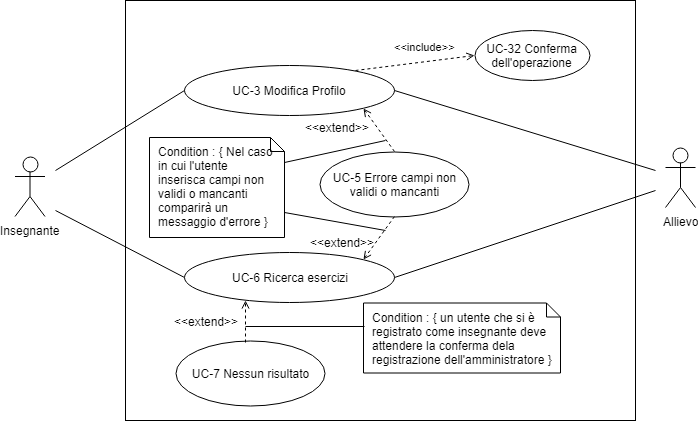
\includegraphics[scale=0.7]{images/UC-3.png}
		\caption{UC-3 Modifica profilo e UC-6 Ricerca esercizi}
	\end{figure}
		
\subsubsection{UC-4 Verifica richiesta insegnante}
		\begin{itemize}
			\item \textbf{Attori:} Moderatore.
			\item \textbf{Precondizione:} Il moderatore si trova nella vista di amministrazione dell'applicazione.
			\item \textbf{Postcondizione:} Il moderatore ha confermato l'utente richiedente il ruolo di insegnante.
			\item \textbf{Scenario principale:}
				\begin{enumerate}
					\item Il moderatore visualizza la lista degli utenti che richiedono il ruolo di insegnante.
					\item Il moderatore accetta o rifiuta l'utente selezionato.
				\end{enumerate}
			\item \textbf{Estensioni:}
			\begin{itemize}
				\item 2.a Il moderatore che verifica la richiesta di insegnante deve confermare o annullare l'operazione (UC-32).
			\end{itemize}
		\end{itemize}

\subsubsection{UC-5 Errore campi non validi o mancanti}
\begin{itemize}
\item \textbf{Attori:} Utente. 
\item \textbf{Precondizione:} L'utente ha inserito dei campi non validi.
\item \textbf{Postcondizione:} Il sistema mostra un messaggio d'errore per spronare l'utente a ricontrollare i campi non validi.
\item \textbf{Scenario principale:}
		\begin{enumerate}
		\item L'utente ha provato a inserire dei campi non validi.
		\item All'utente viene mostrato un messaggio d'errore che invita a ricontrollare i campi non validi.
		\end{enumerate}
\end{itemize}
\subsubsection{UC-6 Ricerca esercizi}
		\begin{itemize}
			\item\textbf{ Attori:} Allievo, insegnante.
			\item \textbf{Precondizione:} L'utente si trova nella vista principale dell'applicazione.
			\item \textbf{Postcondizione:} L'utente ottiene una lista degli esercizi filtrati.
			\item \textbf{Scenario principale:}
				\begin{enumerate}
					\item L'utente accede all'area dedicata alla ricerca degli esercizi.
					\item L'utente scrive la frase nella barra di ricerca.
					\item L'utente seleziona i filtri UC-6.1.
					\item L'utente avvia la ricerca.
				\end{enumerate}
			\item \textbf{Estensioni:}
				\begin{itemize}
					\item 2.a Nel caso in cui l'utente tenti l'inserimento di campi non validi vedrà comparire messaggi d'errore (UC-5).
					\item 3.a Se non c'è nessun risultato viene visualizzato un messaggio: ``nessun risultato trovato" (UC-7).
				\end{itemize}
		\end{itemize}
\subsubsection{UC-6.1 Filtraggio esercizi }
\begin{itemize}
\item \textbf{Attori:} Allievo, insegnante.
			\item \textbf{Precondizione:} L'utente si trova nella vista di ricerca degli esercizi dell'applicazione.
			\item \textbf{Postcondizione:} L'utente ha selezionato i filtri per la ricerca.
			\item \textbf{Scenario principale:}
				\begin{enumerate}
					\item L'utente può selezionare l'autore degli esercizi desiderati.
					\item L'utente può selezionare il livello di difficoltà degli esercizi.
					\item L'utente può selezionare gli argomenti degli esercizi.
				\end{enumerate}

\end{itemize}
\subsubsection{UC-7 Visualizzazione messaggio ``nessun risultato trovato"}
\begin{itemize}
		\item \textbf{Attori:} Insegnante, allievo, sviluppatore.
		
		\item \textbf{Precondizione:} L'utente ha avviato la ricerca. 
		\item \textbf{Postcondizione:} L'utente visualizza un messaggio: ``nessun risultato trovato".
		\item \textbf{Scenario principale: }
		\begin{enumerate}
			\item Viene mostrato un messaggio: ``nessun risultato trovato".
		\end{enumerate}
\end{itemize}

\subsubsection{UC-8 Eliminazione di un utente}
\begin{itemize}
	\item \textbf{Attori:} Moderatore.
	\item \textbf{Precondizione:} Il moderatore si trova nella vista di amministrazione dell'applicazione.
	\item \textbf{Postcondizione:} Il moderatore ha eliminato l'utente desiderato.
	\item \textbf{Scenario principale:}
	\begin{enumerate}
		\item Il moderatore indica l'utente da eliminare.
		\item Il moderatore conferma l'eliminazione dell'utente selezionato.
	\end{enumerate}
\item \textbf{Estensioni:}
\begin{itemize}
	\item 2.a Il moderatore deve confermare o annullare l'operazione di eliminazione utente (UC-32).
\end{itemize}
\end{itemize}

	
\subsubsection{UC-9 Modifica soluzione}
\begin{itemize}
\item \textbf{Attori:} Insegnante.
\item \textbf{Precondizione:} L'insegnante ha selezionato un esercizio di cui ha fornito una soluzione.
\item \textbf{Postcondizione:} La soluzione inserita è stata modificata.
\item \textbf{Scenario principale:}
		\begin{enumerate}
		\item L'insegnante visualizza i campi con la vecchia soluzione.
		\item L'insegnante modifica i campi che ritiene errati.
		\item L'insegnante conferma la modifica.
		\end{enumerate}
	\item \textbf{Estensioni:}
	\begin{itemize}
	\item 3.a L'insegnante che modifica la soluzione di un esercizio deve confermare o annullare l'operazione (UC-32).
	\end{itemize}
\end{itemize}
\begin{figure}[h]
	\centering
	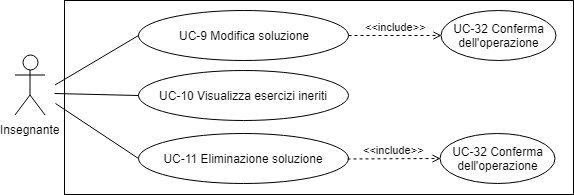
\includegraphics[scale=0.7]{images/UC-9.png}
	\caption{UC-9 Modifica soluzione, UC-10 Visualizzazione esercizi inseriti, UC-11 Eliminare una soluzione di un esercizio}
\end{figure}

\subsubsection{UC-10 Visualizzazione esercizi inseriti}
\begin{itemize}
\item \textbf{Attori: }Insegnante.
		\item \textbf{Precondizione: }L'insegnante si trova nell'area del suo profilo.
		\item \textbf{Postcondizione: }L'insegnante visualizza una lista di esercizi inseriti. 
		\item \textbf{Scenario principale: }
		\begin{enumerate}
		\item L'insegnante accede alla vista degli esercizi inseriti.
		\end{enumerate}
	\end{itemize}
	
\subsubsection{UC-11 Eliminare una soluzione di un esercizio}
\begin{itemize}
\item \textbf{Attori: }Insegnante.
		\item \textbf{Precondizione: }L'insegnate ha selezionato la soluzione da eliminare.
		\item \textbf{Postcondizione: }La soluzione selezionata viene eliminata. 
		\item \textbf{Scenario principale: }
		\begin{enumerate}
		\item L'utente sceglie una soluziona da eliminare.
		\item L'insegnante conferma l'eliminazione.
		\end{enumerate}
	\item Estensioni:
	\begin{itemize}
	\item 2.a L'insegnante che elimina la soluzione di un esercizio puo' confermare o annullare l'operazione (UC-32).
	\end{itemize}
	\end{itemize}

\subsubsection{UC-12 Inserimento esercizio}
	\begin{itemize}
		\item \textbf{Attori: }Insegnante.
		\item \textbf{Precondizione: }L'insegnante è nella vista di inserimento di un nuovo esercizio.
		\item \textbf{Postcondizione: }L'esercizio è stato inserito.
		\item \textbf{Scenario principale: }
		\begin{enumerate} 
		\item L'insegnante inserisce la frase.
		\item L'insegnante inserisce la soluzione UC-12.1.
		\item L'insegnante inserisce la difficoltà.
		\item L'insegnante inserisce gli argomenti UC-12.2.
		\item L'insegnante conferma l'inserimento.
		\end{enumerate}
		\item \textbf{Estensioni:} 
		\begin{itemize}
			\item 5.a Un insegnante che inserisce un esercizio deve confermare o annullare l'operazione (UC-32).
		\item 6.a Nel caso in cui i campi compilati presentino errori verrà mostrato un messaggio d'errore (UC-5).
		\end{itemize}
	\end{itemize}
	\begin{figure}[h]
	\centering
	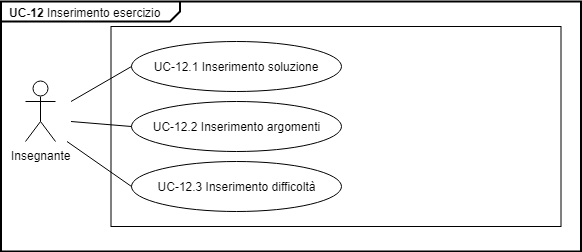
\includegraphics[scale=0.7]{images/UC-12.png}
	\caption{UC-12 Inserimento esercizio}
\end{figure}

\subsubsection{UC-12.1 Inserimento di una soluzione}
\begin{itemize}
\item \textbf{Attori: }Insegnante.
\item \textbf{Precondizione: }L'insegnante è nella vista di inserimento di un nuovo esercizio.
\item \textbf{Postcondizione: }L'insegnante ha inserito la propria soluzione.
\item \textbf{Scenario principale: }
		\begin{enumerate} 
		\item L'insegnante visualizza i campi proposti dal generatore automatico. 
		\item L'insegnante può modificare i campi che ritiene errati.
		\item L'insegnante seleziona lo stato della soluzione inserita, pubblica o privata.
		\item L'insegnante conferma la soluzione.
		\end{enumerate}	
	\item \textbf{Estensioni:}
	\begin{itemize}
	\item 4.a Un insegnante che inserisce una soluzione deve confermare o annullare l'operazione (UC-32).
	\end{itemize}
\end{itemize}

\subsubsection{UC-12.2 Inserimento argomenti}
\begin{itemize}
\item \textbf{Attori: }Insegnante.

\item \textbf{Precondizione:} L'insegnante sta inserendo un esercizio, gli viene richiesta la compilazione di una lista di argomenti presenti nell'esercizio.
\item \textbf{Postcondizione:} L'insegnante ha selazionato gli argomenti trattati nell'esercizio.
\item \textbf{Scenario principale: }
		\begin{enumerate}
		\item L'insegnante sta inserendo un esercizio. 
		\item L'insegnante seleziona gli argomenti che vengono toccati nell'esercizio. 
		\end{enumerate}
\end{itemize}				

	\subsubsection{UC-13 Svolgimento esercizio}
	\begin{itemize}
	\item \textbf{Attori:} Allievo.
			\item \textbf{Precondizione:}  L'allievo visualizza la lista degli esercizi ricercati.
			\item \textbf{Postcondizione:} L'allievo visualizza la valutazione dell'esercizio.
			\item \textbf{Scenario principale:}
			\begin{enumerate}
				\item l'allievo seleziona l'esercizio da svolgere (UC-13.1).
				\item l'allievo compila i campi (UC-13.2).
				\item l'allievo conferma i dati inseriti.
				\item l'allievo visualizza la valutazione (UC-13.3).
			\end{enumerate}
		\item \textbf{Estensioni:}
		\begin{itemize}
			\item 3.a Un allievo che invia i dati per lo svolgimento dell'esercizio deve confermare o annullare l'operazione (UC-32).
		\end{itemize}
	\end{itemize}
	\begin{figure}[h]
		\centering
		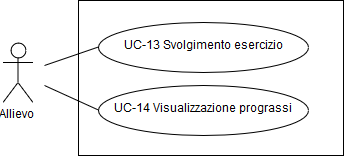
\includegraphics[scale=0.7]{images/UC-13.png}
		\caption{UC-13 Svolgimento esercizio, UC-14 Visualizzazione progressi}
	\end{figure}	
			
	\subsubsection{UC-13.1 Selezione esercizio}
	\begin{itemize}
			\item \textbf{Attori:} Allievo.
			\item \textbf{Precondizione:} L'allievo visualizza la lista degli esercizi ricercati.
			\item \textbf{Postcondizione:} L'allievo visualizza la vista per l'esecuzione dell'esercizio.
			\item \textbf{Scenario principale:}
				\begin{enumerate}
					\item l'allievo seleziona la frase da svolgere.
					\item l'allievo seleziona il correttore dell'esercizio(insegnante o algoritmo automatico).
					\item l'allievo conferma la selezione.
				\end{enumerate}
			\item \textbf{Estensioni:}
			\begin{itemize}
		\item 3.a Un allievo che indica l'esercizio e il correttore  deve confermare o annullare l'operazione (UC-32).
			\end{itemize}
			\end{itemize}
			\begin{figure}[h]
		\centering
		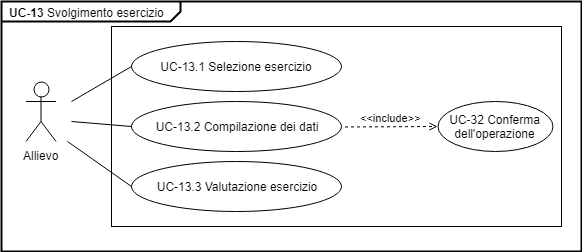
\includegraphics[scale=0.7]{images/UC-13_1.png}
		\caption{UC-13.1 Selezione esercizio, UC-13.2 Compilazione dei dati, UC-13.3 Valutazione esercizio}
	\end{figure}

	\subsubsection{UC-13.2 Compilazione dei campi}
		\begin{itemize}
			\item \textbf{Attori:} Allievo.
			\item \textbf{Precondizione:} L'allievo ha selezionato un esercizio da eseguire.
			\item \textbf{Postcondizione:} L'allievo ha compilato i campi proposti dall'esercizio.
			\item \textbf{Scenario principale:}
				\begin{enumerate}
					\item L'allievo sceglie la classe grammaticale per ogni parola presentata.
					\item L'allievo conferma la soluzione dell'esercizio.
				\end{enumerate}
			\item \textbf{Estensioni:} 
				\begin{itemize}
					\item 2.a Un allievo dopo la compilazione dei campi deve confermare o annullare l'operazione (UC-32).
					\item 2.b Nel caso in cui l'utente tenti l'inserimento di campi non validi vedrà comparire messaggi d'errore (UC-5).
				\end{itemize}
		\end{itemize}

	\subsubsection{UC-13.3 Valutazione esercizio}
	\begin{itemize}
			\item \textbf{Attori:} Allievo.
			\item \textbf{Precondizione:} L'allievo ha completato l'esecuzione dell'esercizio.
			\item \textbf{Postcondizione:} L'allievo visualizza la valutazione dell'esercizio.
			\item \textbf{Scenario principale:}
				\begin{enumerate}
					\item L'allievo al termine dell'esecuzione dell'esercizio riceve la valutazione.
				\end{enumerate}
			\end{itemize}
			
	\subsubsection{UC-14 Visualizzazione progressi}
	\begin{itemize}
			\item \textbf{Attori:} Allievo.
			\item \textbf{Precondizione:} L'allievo si trova nella vista del proprio profilo.
			\item \textbf{Postcondizione:} L'allievo visualizza i progressi svolti fino a quel momento.
			\item \textbf{Scenario principale:}
				\begin{enumerate}
					\item L'allievo visualizza la media delle valutazioni ricevute.
					\item L'allievo visualizza i grafici riguardanti i propri progressi.
					\item L'allievo visualizza il numero di esercizi svolti.
				\end{enumerate}
	\end{itemize}